\documentclass[a4paper,11pt]{article}
\usepackage{xeCJK}
\usepackage[margin=1.8cm]{geometry}
\usepackage{tikz}
\usetikzlibrary{positioning, shadows, calc, arrows.meta, angles, quotes}
\usepackage{amsmath,amssymb}
\usepackage{multicol}
\usepackage{enumitem}
\usepackage{fancyhdr}
\usepackage{xcolor}
\usepackage[most]{tcolorbox}
\usepackage{fontspec}
\usepackage{lmodern}

% 設定字體
\setCJKmainfont[
  Path={./assets/fonts/},
  Extension=.otf, % 假設字體是 .otf, 根據實際情況調整
  BoldFont=SourceHanSansTC-Bold, % 確保這些字體文件名存在於指定路徑
  ItalicFont=SourceHanSansTC-Regular, % 示例,可能沒有斜體
  BoldItalicFont=SourceHanSansTC-Bold % 示例
]{SourceHanSansTC-Regular}
\setmainfont[
  Path={./assets/fonts/},
  Extension=.otf,
  BoldFont=SourceHanSansTC-Bold
]{SourceHanSansTC-Regular}
\setmonofont[
  Path={./assets/fonts/},
  Extension=.otf
]{SourceHanSansTC-Regular}

% 全局字體設置
\renewcommand{\normalsize}{\fontsize{10pt}{14pt}\selectfont} % 稍小一點以容納更多圖形
\pagestyle{fancy}
\fancyhf{}
\renewcommand{\headrulewidth}{0pt}
\fancyfoot[C]{\thepage}
\setlength{\parskip}{0.5em}
\setlength{\parindent}{0em}
\setlist[enumerate]{leftmargin=*,labelsep=0.5em,topsep=0.3em,itemsep=0.2em}
\definecolor{sectioncolor}{rgb}{0.2,0.4,0.6}
\usepackage{titlesec}
\titleformat{\subsection}[block]{\large\bfseries\color{sectioncolor}}{\thesubsection}{1em}{\centering}
\titlespacing*{\subsection}{0pt}{3.5ex plus 1ex minus .2ex}{2.3ex plus .2ex}

\title{\Huge PredefinedTriangleGenerator 畫廊}
\author{}
\date{}

\begin{document}
\maketitle
\thispagestyle{empty}
\centering

\subsection*{SSS (3-4-5) - 僅輪廓和頂點名}


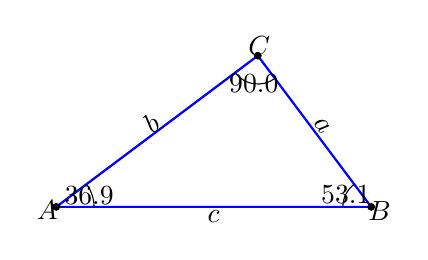
\begin{tikzpicture}[scale=0.8] % 調整 scale 以適應頁面

\draw[blue, thick] (0,0) -- (5,0) -- (3.2,2.4) -- cycle;
\filldraw[black] (0,0) circle (1.5pt);
\node[anchor=center, color=black] at (-0.1423025,-0.04743416) {$A$};
\filldraw[black] (5,0) circle (1.5pt);
\node[anchor=center, color=black] at (5.134164,-0.06708204) {$B$};
\filldraw[black] (3.2,2.4) circle (1.5pt);
\node[anchor=center, color=black] at (3.221213,2.548492) {$C$};
\node[anchor=center, rotate=0, color=black] at (2.5,-0.15) {$c$};
\node[anchor=center, rotate=-53.1301, color=black] at (4.22,1.29) {$a$};
\node[anchor=center, rotate=36.8699, color=black] at (1.51,1.32) {$b$};
\draw[thin] (0.6,0) arc (0:36.8699:0.6);
\node[anchor=center, rotate=0, color=black] at (0.5217758,0.1739253) {$36.9°$};
\draw[thin] (4.73,0.36) arc (126.8699:180:0.45);
\node[anchor=center, rotate=0, color=black] at (4.597508,0.2012461) {$53.1°$};
\draw[thin] (2.84,2.13) arc (-143.1301:-53.1301:0.45);
\node[anchor=center, rotate=0, color=black] at (3.13636,1.954523) {$90.0°$};

\end{tikzpicture}

\newpage

\subsection*{座標定義 - 顯示邊長和P1角}


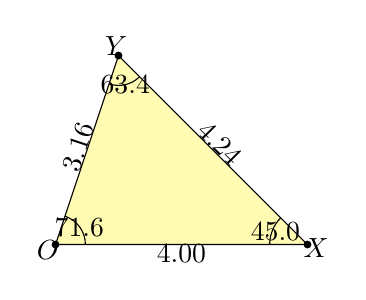
\begin{tikzpicture}[scale=0.8] % 調整 scale 以適應頁面

\draw[thin, black, fill=yellow!30] (0,0) -- (4,0) -- (1,3) -- cycle;
\filldraw[black] (0,0) circle (1.5pt);
\node[anchor=center, color=black] at (-0.1216863,-0.08770654) {$O$};
\filldraw[black] (4,0) circle (1.5pt);
\node[anchor=center, color=black] at (4.138582,-0.05740251) {$X$};
\filldraw[black] (1,3) circle (1.5pt);
\node[anchor=center, color=black] at (0.9655371,3.145987) {$Y$};
\node[anchor=center, rotate=0, color=black] at (2,-0.15) {4.00};
\node[anchor=center, rotate=-45, color=black] at (2.606066,1.606066) {4.24};
\node[anchor=center, rotate=71.56505, color=black] at (0.3576975,1.547434) {3.16};
\draw[thin] (0.4743416,0) arc (0:71.56505:0.4743416);
\node[anchor=center, rotate=0, color=black] at (0.3782236,0.2726082) {$71.6°$};
\draw[thin] (3.575736,0.4242641) arc (135:180:0.6);
\node[anchor=center, rotate=0, color=black] at (3.491866,0.2104759) {$45.0°$};
\draw[thin] (0.85,2.55) arc (-108.4349:-45:0.4743416);
\node[anchor=center, rotate=0, color=black] at (1.107117,2.546244) {$63.4°$};

\end{tikzpicture}

\newpage

\subsection*{SAS (4, 60deg, 3) - 顯示所有角和質心}


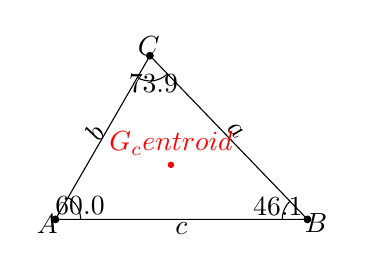
\begin{tikzpicture}[scale=0.8] % 調整 scale 以適應頁面

\draw[thin, black] (0,0) -- (4,0) -- (1.5,2.598076) -- cycle;
\filldraw[black] (0,0) circle (1.5pt);
\node[anchor=center, color=black] at (-0.1299038,-0.075) {$A$};
\filldraw[black] (4,0) circle (1.5pt);
\node[anchor=center, color=black] at (4.138023,-0.05873269) {$B$};
\filldraw[black] (1.5,2.598076) circle (1.5pt);
\node[anchor=center, color=black] at (1.481852,2.746974) {$C$};
\node[anchor=center, rotate=0, color=black] at (2,-0.15) {$c$};
\node[anchor=center, rotate=-46.10211, color=black] at (2.858087,1.403044) {$a$};
\node[anchor=center, rotate=60, color=black] at (0.6200962,1.374038) {$b$};
\draw[thin] (0.4,0) arc (0:60:0.4);
\node[anchor=center, rotate=0, color=black] at (0.3897114,0.225) {$60.0°$};
\draw[thin] (3.72265,0.2882307) arc (133.8979:180:0.4);
\node[anchor=center, rotate=0, color=black] at (3.530209,0.1999085) {$46.1°$};
\draw[thin] (1.3,2.251666) arc (-120:-46.10211:0.4);
\node[anchor=center, rotate=0, color=black] at (1.554443,2.151382) {$73.9°$};
\filldraw[red] (1.833333,0.8660254) circle (1.2pt);
\node[anchor=south, color=red] at (1.833333,0.8660254) {$G_centroid$};

\end{tikzpicture}

\newpage

\subsection*{ASA (30deg, 5, 70deg) - 顯示邊名和內心}


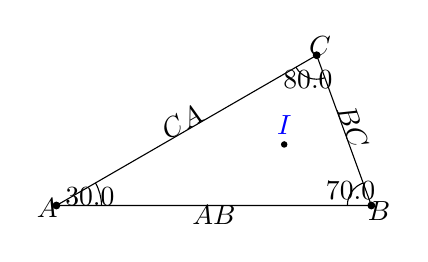
\begin{tikzpicture}[scale=0.8] % 調整 scale 以適應頁面

\draw[thin, black] (0,0) -- (5,0) -- (4.131759,2.385472) -- cycle;
\filldraw[black] (0,0) circle (1.5pt);
\node[anchor=center, color=black] at (-0.1448889,-0.03882286) {$A$};
\filldraw[black] (5,0) circle (1.5pt);
\node[anchor=center, color=black] at (5.122873,-0.08603647) {$B$};
\filldraw[black] (4.131759,2.385472) circle (1.5pt);
\node[anchor=center, color=black] at (4.183062,2.526426) {$C$};
\node[anchor=center, rotate=0, color=black] at (2.5,-0.15) {$AB$};
\node[anchor=center, rotate=-70, color=black] at (4.706833,1.244039) {$BC$};
\node[anchor=center, rotate=30, color=black] at (1.99088,1.32264) {$CA$};
\draw[thin] (0.7156417,0) arc (0:30:0.7156417);
\node[anchor=center, rotate=0, color=black] at (0.5312592,0.1423505) {$30.0°$};
\draw[thin] (4.869764,0.3578208) arc (110:180:0.380785);
\node[anchor=center, rotate=0, color=black] at (4.66918,0.2316427) {$70.0°$};
\draw[thin] (3.80199,2.19508) arc (-150:-70:0.380785);
\node[anchor=center, rotate=0, color=black] at (3.993632,2.005971) {$80.0°$};
\filldraw[black] (3.616189,0.9689549) circle (1.2pt);
\node[anchor=south, color=blue] at (3.616189,0.9689549) {$I$};

\end{tikzpicture}

\newpage

\subsection*{AAS (45deg, 60deg, side opp A = 4) - 顯示自定義標籤}


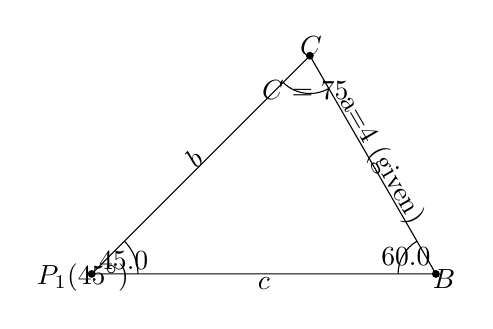
\begin{tikzpicture}[scale=0.8] % 調整 scale 以適應頁面

\draw[thin, black] (0,0) -- (5.464102,0) -- (3.464102,3.464102) -- cycle;
\filldraw[black] (0,0) circle (1.5pt);
\node[anchor=center, color=black] at (-0.1385819,-0.05740251) {$P_1 (45^\circ)$};
\filldraw[black] (5.464102,0) circle (1.5pt);
\node[anchor=center, color=black] at (5.594005,-0.075) {$B$};
\filldraw[black] (3.464102,3.464102) circle (1.5pt);
\node[anchor=center, color=black] at (3.483681,3.612818) {$C$};
\node[anchor=center, rotate=0, color=black] at (2.732051,-0.15) {$c$};
\node[anchor=center, rotate=-60, color=black] at (4.594005,1.807051) {a=4 (given)};
\node[anchor=center, rotate=45, color=black] at (1.625985,1.838117) {$b$};
\draw[thin] (0.7348469,0) arc (0:45:0.7348469);
\node[anchor=center, rotate=0, color=black] at (0.5081337,0.2104759) {$45.0°$};
\draw[thin] (5.164102,0.5196152) arc (120:180:0.6);
\node[anchor=center, rotate=0, color=black] at (4.987788,0.275) {$60.0°$};
\draw[thin] (3.039838,3.039838) arc (-135:-60:0.6);
\node[anchor=center, rotate=0, color=black] at (3.392312,2.918807) {$C=75°$};

\end{tikzpicture}

\vspace{1cm}


\end{document}
